\section{Revision on Compiling Phases}
The MT22-MIPS compiler converts a source program in the MT22 language to a program in a MIPS assembly.

\begin{figure}[ht]
    \centering
    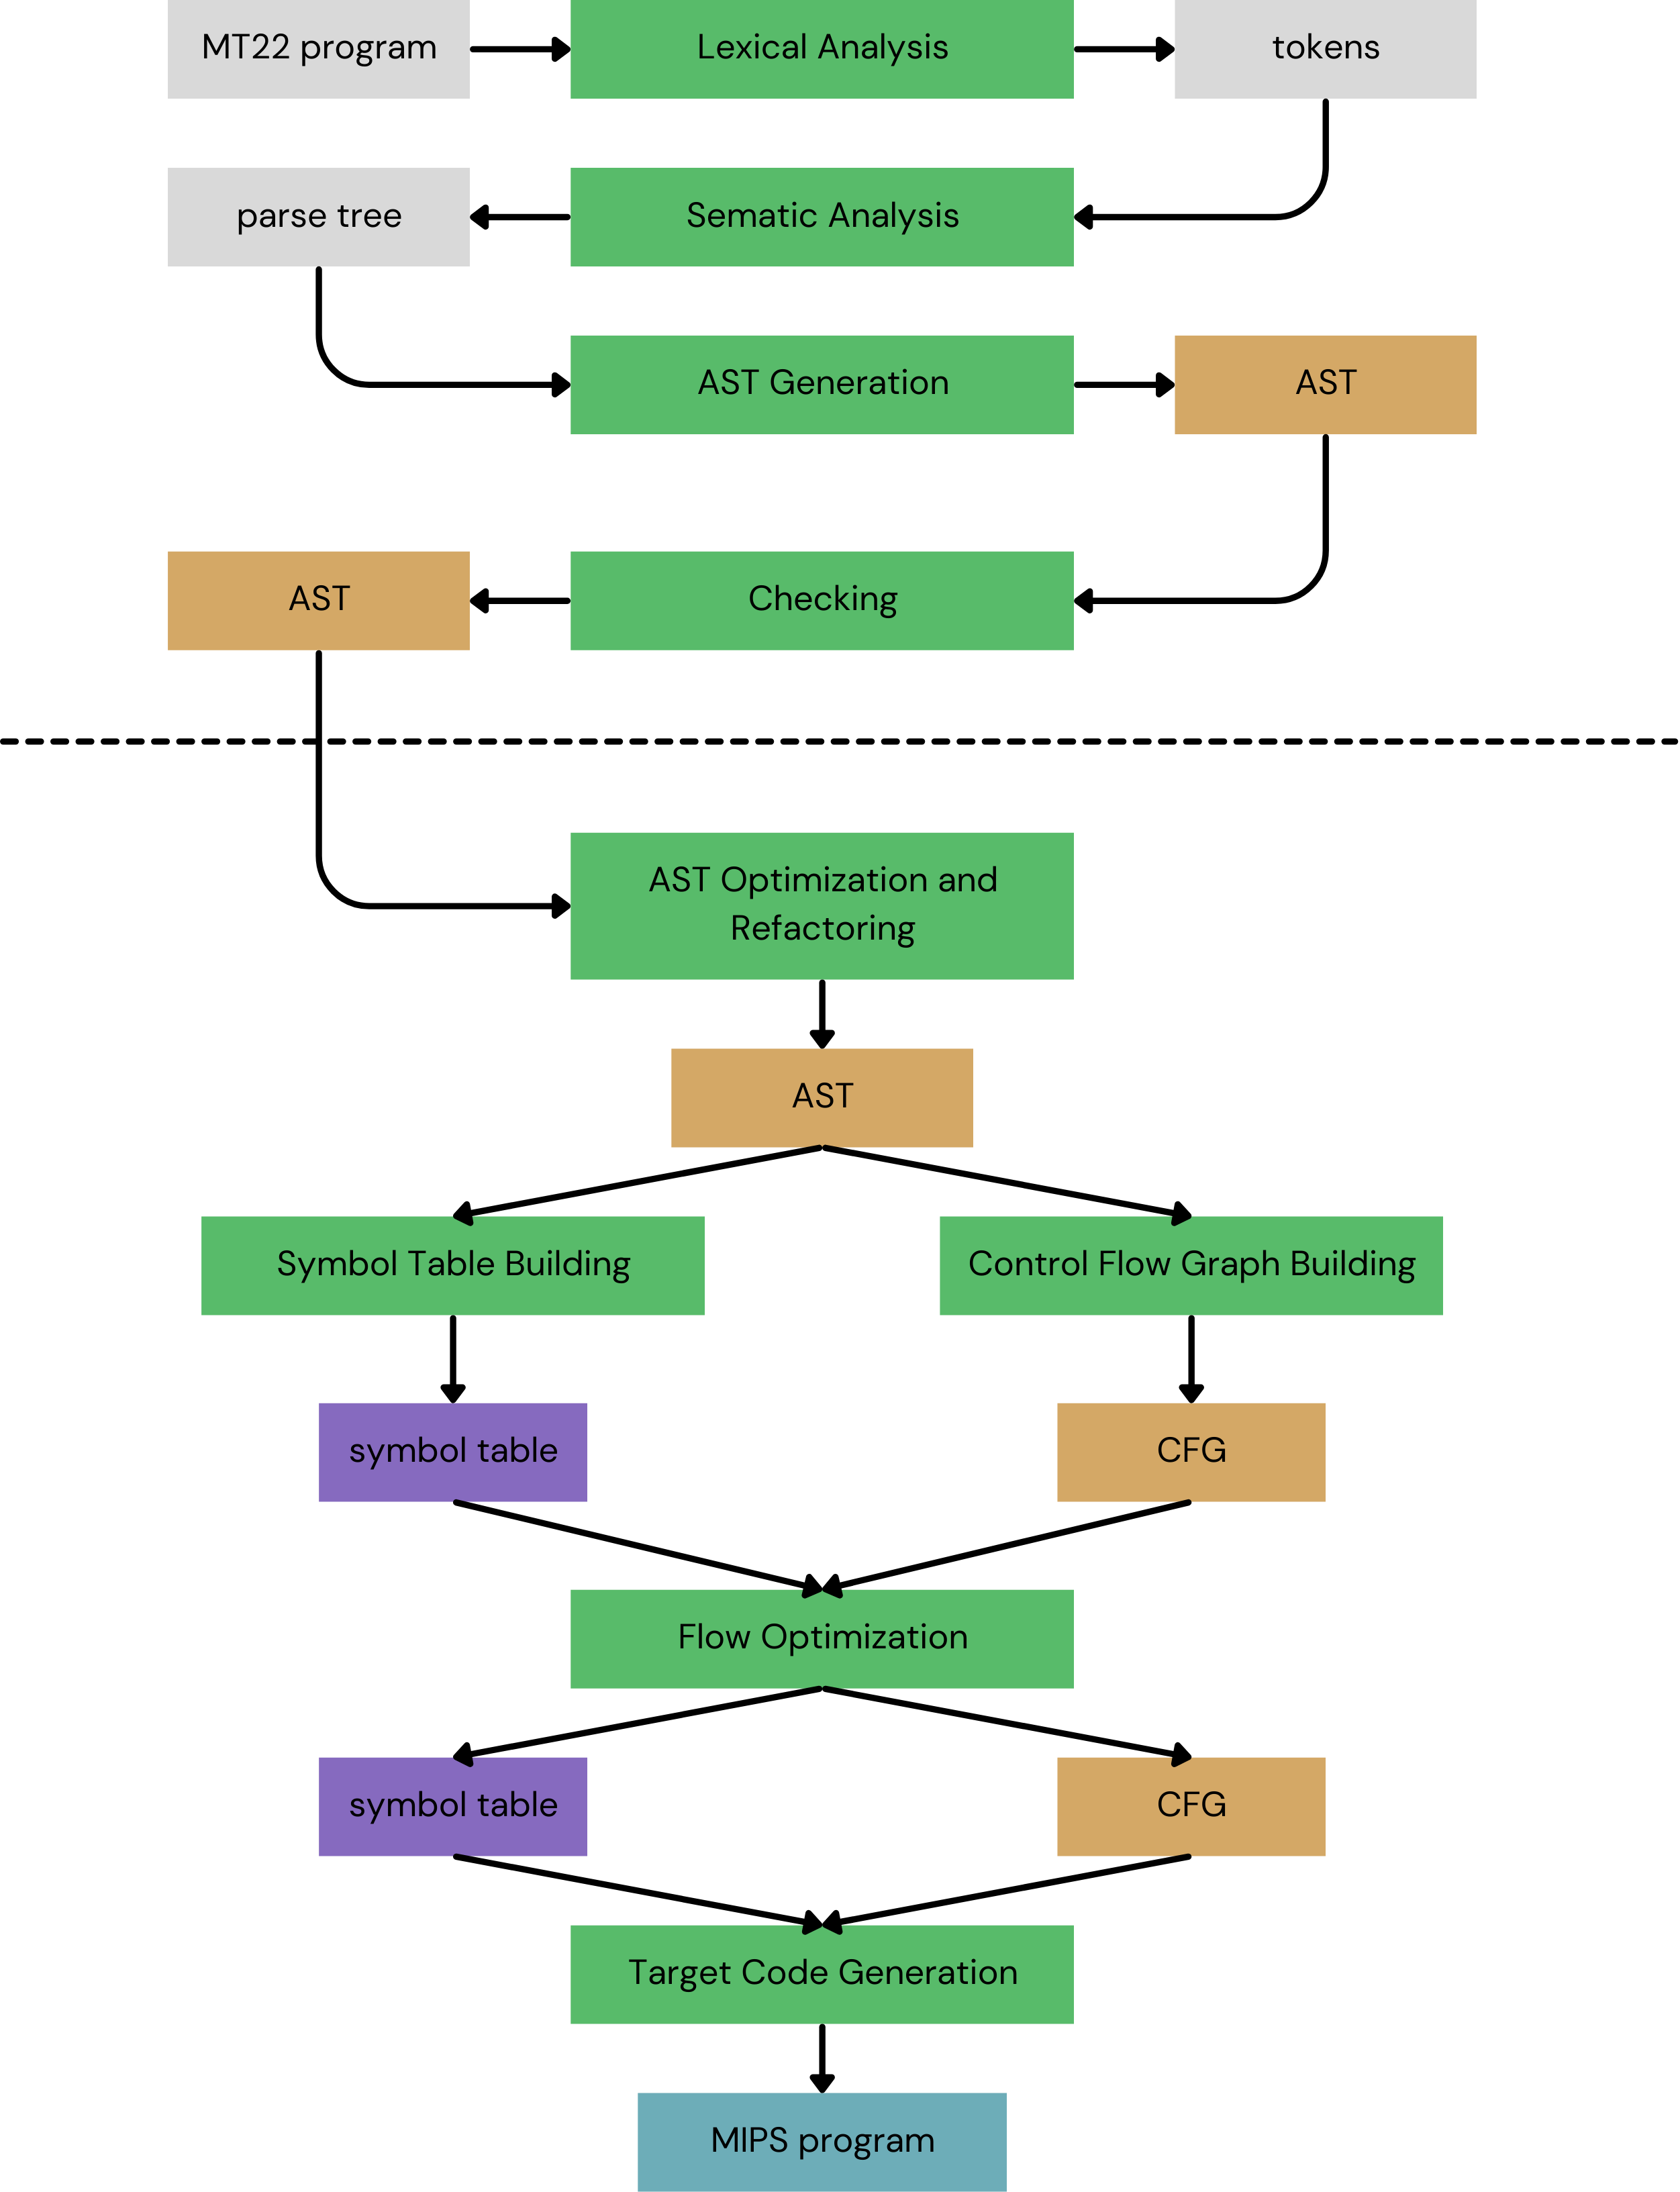
\includegraphics[width=0.8\textwidth]{img/compiler-phases.png}
    \caption{Phases of MT22-MIPS compiler}
    \label{figure:compiler-phases}
\end{figure}

Figure \ref{figure:compiler-phases} illustrates phases of the MT22-MIPS compiler, derived closely to general compilers. The dashed line separates between frontend and backend processes. The frontend has been implemented in class assignments. Here we focus on the backend. Abstract Syntax Tree (AST) is a well-known intermediate representation (IR) for our program, whose major nodes are shown in Figure \ref{figure:ast}. Note that BlockStmt, IfStmt, ForStmt, WhileStmt and DoWhileStmt include at least one Stmt. The AST is produced after the frontend process, then it is refactored and optimized one more time in the backend.

\begin{figure}[ht]
    \centering
    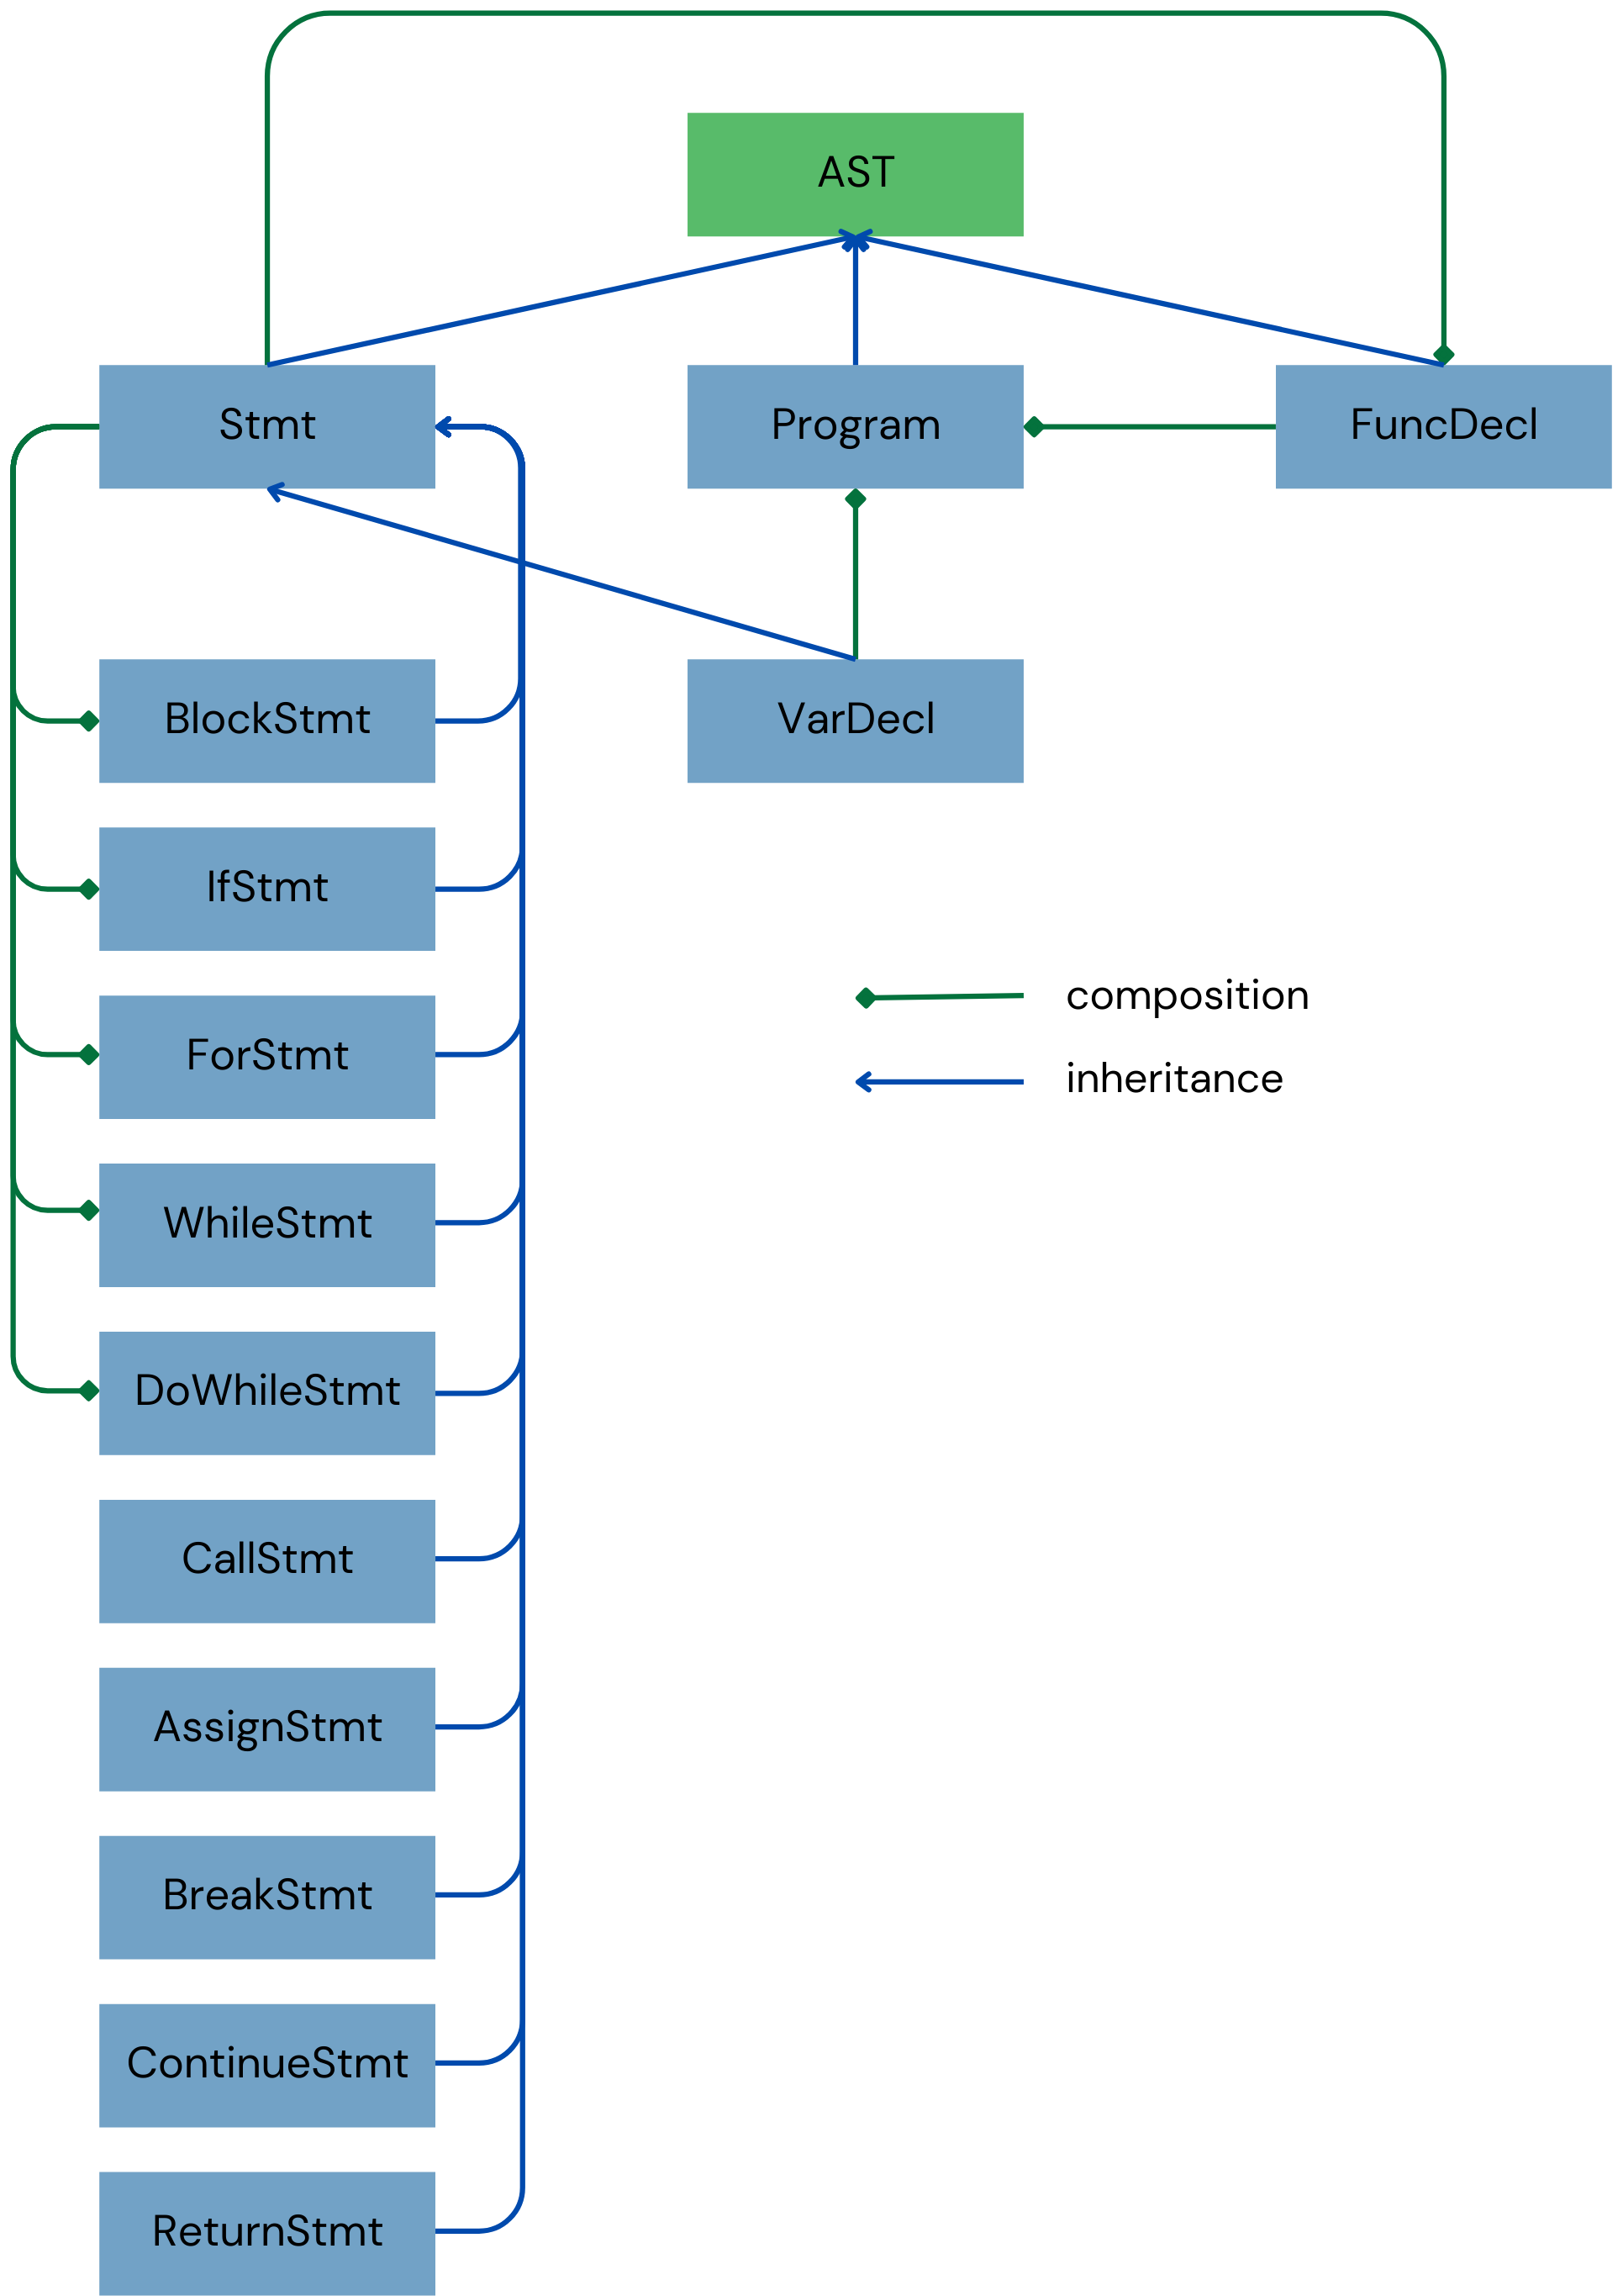
\includegraphics[width=0.7\textwidth]{img/ast.png}
    \caption{Overview of statement relations}
    \label{figure:ast}
\end{figure}

Another equivalent IR, the Control Flow Graph (CFG) and an assisting data structure, the Symbol Table. Flow Optimization and Target Code Generation work with the symbol table and the CFG.